\documentclass[../thesis.tex]{subfiles}

\begin{document}

\chapter{Implementierung}
\label{chp: implementierung}
In \autoref{chp: grundlagen} wurde die in \cite{jaubert2020benchmark} entwickelte Methode zur Bewertung binärer Gemische dargestellt und um sinnvolle Randbedingungen bei der Notenberechnung ergänzt. In diesem Kapitel geht es um die softwaremäßige Umsetzung des vorgestellten Benchmarks.
Um die Bewertung einer Zustandsgleichung vornehmen zu können, sind einige Voraussetzungen zu erfüllen. Die experimentellen Daten müssen zur Verfügung stehen und die Daten des Modells müssen, sofern das möglich ist, berechnet und anschließend mit denen der Experimente verglichen werden. Das Ergebnis der Bewertung ist eine Notenzusammenstellung.

Da die im Zusatzmaterial von \cite{jaubert2020benchmark} zur Verfügung gestellte Excel Datei sich nur schwer nach den für den Vergleich notwendigen Daten und Parametern durchsuchen lässt, werden die experimentellen Daten in ein anderes Format überführt. Um den Vergleich zu vereinfachen, wird für die gespeicherten Modelldaten das gleiche Format verwendet. Um mehrere durchgeführte Benchmarks miteinander vergleichen zu können, werden auch die Ergebnisse in einer Datei gespeichert. Aus dem vorgestellten Vorgehen ergeben sich drei voneinander unabhängige Problemstellungen die zur Durchführung des Benchmarks gelöst werden müssen.

\begin{enumerate}
	\item Aufbereitung der experimentellen Daten
	\item Berechnung der Modelldaten
	\item Durchführung des Benchmarks
\end{enumerate}

Die Aufbereitung der experimentellen Daten muss einmalig geschehen, wenn die notwendige Infrastruktur aufgesetzt wird. Zur Berechnung der Modelldaten müssen die experimentellen Daten im aufbereiteten Format vorliegen, damit die dort verwendeten Parameter eingelesen und für die Modellrechnung verwendet werden können. Wenn sowohl die experimentellen Daten als auch die Modellwerte vorliegen, kann der Vergleich durchgeführt werden. In den nun folgenden Abschnitten wird das genauere Vorgehen zur Lösung der aufgezählten Problemstellungen beschrieben. Der gesamte Quellcode, welcher zur Durchführung des Benchmarks benötigt wird, ist im Ordner \texttt{Software/dev} zu finden. 

\section{Datenbank}

Die Klasse \texttt{database} dient zur Bereitstellung und Speicherung der experimentellen Daten. Die Klasse Datenbank erzeugt für jedes Gemisch eine eigene Datei, in der alle Daten im \texttt{.json} Format abgelegt sind. Dieses gewählte Dateiformat lässt die Ablage der Daten in einer hierarchischen Struktur zu, was die spätere Verwendung vereinfacht. Zusätzlich lässt sich eine solche Datei in menschenlesbarem Format speichern und anzeigen, was die Fehlersuche bei der Entwicklung leichter gestaltet. Die Dateien werden im Ordner \texttt{Datenbank/Experimente} abgelegt. Der beispielhafte Aufbau einer Gemischdatei ist in \autoref{code: beispielgemisch} dargestellt. Da nicht für alle binären Gemische alle Daten zur Verfügung stehen, werden in einer solchen Datei bloß die Werte angelegt, zu denen es Messreihen gibt.

\definecolor{codehighlight}{rgb}{0.95,0.8,0.8}
\lstinputlisting[language=Python, caption=Gemischdatei Beispiel, basicstyle=\fontsize{7}{8}\selectfont\ttfamily
]{./code/gemischbeispiel.json}
\label{code: beispielgemisch}

Der Schlüssel \texttt{BAC} dient der Klassifizierung des Gemisches, wie in Listing \autoref{sec: gemischklassifikation} beschrieben. Das Tabellenblatt, auf dem die Daten in der Originaldatei zu finden sind, ist als Wert des Schlüssels \texttt{sheet} gespeichert. Analog zum Aufbau der Originaldatei werden unter den weiteren Schlüsseln die Daten der gemessenen Größen gespeichert. Alle Messreihen werden als Liste unter dem jeweiligen Variablennamen gespeichert.

Eine Messreihe ist durch ihre Quelle unter dem Punkt \texttt{reference}, die Parameter der Messung unter dem Punkt \texttt{params} und die Messdaten unter dem Punkt \texttt{measurements} charakterisiert. Die Parameter einer Messung können im Falle eines isobaren Phasengleichgewichts der Druck $ p $ oder im Falle der Mischungswärmekapazität der Druck $ p $ und die Temperatur $ T $ sein. Diese Werte werden zur Berechnung der jeweiligen Zielgröße gebraucht. 

Somit stehen alle experimentellen Daten in computerlesbarem Format zur Verfügung. Die Datenbank muss, wie bereits erwähnt, einmalig erzeugt werden, was ein Aufruf der Testdatei \texttt{test\_database.py} erledigt.

\section{Modell}

Die Klasse \texttt{model} dient dazu die Daten des Modells bereitzustellen, damit diese anschließend mit den experimentellen Daten verglichen und bewertet werden können.

Der Ablauf der Berechnung für ein Gemisch ist in \autoref{fig: model_berechnung} gezeigt.

\begin{figure}[htb]
	\centering
	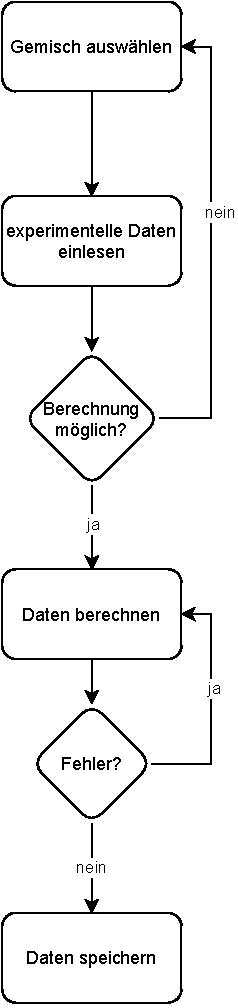
\includegraphics[scale=0.9]{berechnung_model}
	\caption{Ablauf Berechnung Model}
	\label{fig: model_berechnung}
\end{figure}

Für jedes Gemisch werden die folgenden Schritte für jede zu berechnende Größe durchgeführt. Zunächst wird das zu berechnende Gemisch festgelegt. Dies geschieht anhand der Reihenfolge, in welcher die Dateien im Ordner liegen und somit alphabetisch nach dem Namen der ersten beteiligten Komponente. Anschließend werden alle vorhandenen experimentellen Daten aus der entsprechenden \texttt{.json} Datei eingelesen. Die hier eingelesenen Daten bestimmen, was das Modell berechnen soll. Es werden alle Bewertungsgrößen, die für das Gemisch gefunden wurden, nacheinander berechnet. Um eine Bewertungsgröße mit dem Modell berechnen zu können, wird die erste Messreihe für diese Größe eingelesen und deren Parameter bestimmt. Die Parameter mit den Daten des Experiments beinhalten alle Daten, die für das Modell notwendig sind, um die Zielgröße berechnen zu können.

Bevor das Modell aufgerufen wird, wird getestet ob das Modell die Daten für das Gemisch berechnen kann. Dieser Test basiert auf den Parametern, die für das Modell vorhanden sind. Diese Parameter können beispielsweise kritische Stoffgrößen wie der kritische Druck $p_\mathrm{c}$, die kritische Temperatur $T_\mathrm{c}$ oder aber modellspezifische Parameter wie $c_1$, $c_2$ und $c_3$ im Fall der \texttt{PSRK} sein. Der Test der Berechenbarkeit ist nicht zwingend notwendig. Er erspart aber einigen Rechenaufwand, da ein Fehler bei der Berechnung vorhersehbar ist. Gerade bei iterativ rechnenden Methoden wie z.B. die Phasengleichgewichtsberechnung kann so nicht notwendige Rechenzeit eingespart werden. Ist ein Stoff an dem Gemisch beteiligt, für den das Modell keine Parameter hat, wird das Gemisch übersprungen.
Sind alle Voraussetzungen für die Berechnung mit dem Modell erfüllt, wird es aufgerufen und die Ergebnisse bei fehlerfreier Rechnung gespeichert. Der Speichervorgang ist hilfreich, um nicht bei jeder Durchführung des Benchmarks die Daten des Modells erneut berechnen zu müssen, da dies sehr zeitaufwendig ist. Falls ein Fehler auftritt, wird versucht den nächsten Datenpunkt der Messreihe zu berechnen. Die Datei mit den Berechnungsergebnissen des Modells hat den gleichen Aufbau, wie die der experimentellen Daten aus Listing \autoref{code: beispielgemisch}. Alle Modellergebnisse werden unter dem Ordner \texttt{Datenbank/Modelle/<Modellname>} gespeichert.

Die Klasse \texttt{model} kann die Daten des Experiments mit den Berechnungsergebnissen des Modells in einem Phasendiagramm darstellen. Alle für die Gemische erzeugten Phasendiagramme sind im Ordner \texttt{Diagramme/<Modellname>} zu finden. Die das Phasendiagramm charakterisierenden Parameter (Druck oder Temperatur) sowie die beteiligten Stoffe, können dem Dateinamen des Diagramms entnommen werden. Im Falle eines isothermen Phasendiagramms sind neben den beteiligten Komponenten die Temperatur in K und im Falle eines isobaren Phasendiagramms der Druck in bar im Dateinamen zu finden.

\section{Bewertung}

Die Klasse Bewertung dient dazu, die experimentellen Daten mit den Modelldaten zu vergleichen und die Bewertung der resultierenden Abweichungen durchzuführen. Als Ergebnis werden die Teilnoten der betrachteten Systeme, BACs und Klassen, sowie die Gesamtnote des Modells berechnet. Die Modellergebnisse sind im Ordner
\newline \texttt{Ergebnisse/<Modellname>} zu finden. In der zu dem Text gehörenden \texttt{.json} Datei sind sowohl die Gesamtergebnisse der Klassen und des Modells, sowie die Einzelergebnisse der beteiligten Systeme hierarchisch aufgeführt. Die beispielhafte Struktur einer solchen Ergebnisdatei ist in Listing \autoref{code: ergebnisbeispiel} dargestellt.

\definecolor{codehighlight}{rgb}{0.95,0.8,0.8}
\lstinputlisting[language=Python, caption=Ergebnisdatei Beispiel, basicstyle=\fontsize{7}{8}\selectfont\ttfamily
]{./code/ergebnisbeispiel.json}
\label{code: ergebnisbeispiel}

Die Ergebnisdatei weist eine hierarchische Struktur auf. Für jeden BAC werden unter dem Schlüssel \texttt{sys\_res} die Teilnoten der einzelnen Systeme gespeichert. Die aus den Teilnoten berechneten Ergebnisse des einzelnen BACs sind unter \texttt{group\_res} zu finden. Die Gesamtnote des BACs ist in \texttt{res} gespeichert. Die Klassenergebnisse, welche die Ergebnisse der einzelnen BACs weiter zusammenfassen sind unter dem Schlüssel \texttt{class\_res} gespeichert. Das Gesamtergebnis des Modells ist unter \texttt{model\_res} zu finden. Beim Berechnen der Noten für die verschiedenen Bewertungsgrößen kommt es zu einigen Schwierigkeiten. Für die implementierten Größen werden diese in den folgenden Abschnitten beschrieben und die vorgesehenen Lösungen erläutert.

\subsection{Bewertung Mischungswärmekapazität und Mischungsenthalpie}

Für die Mischungswärmekapazität werden die berechneten Daten mit den experimentellen Daten wie in \autoref{eq: cp MAPEs} beschrieben verglichen. Sollte eine Berechnung für ein Gemisch aufgrund eines Fehler nicht möglich sein, betrifft dieser immer die gesamte Messreihe oder das gesamte Gemisch. Da für alle experimentellen Datensätze einer Messreihe Werte berechnet werden können, ist gewährleistet, dass die Anzahl der zur Verfügung stehenden experimentellen Daten mit der Anzahl der aus dem Modell erhaltenen übereinstimmt.

Dies stimmt auch für die Mischungsenthalpie.

\subsection{Bewertung Phasengleichgewichte}

Für die Bewertung der Phasengleichgewichte müssen die Daten des Modells und die experimentellen Daten zusammengeführt werden. Das Modell berechnet typischerweise eine weitaus größere Anzahl an Datenpunkten als im experimentellen Datensatz vorliegen. Das liegt an der verwendeten \texttt{TREND} Methode \texttt{PTXDIAG\_FIT}. Diese Methode berechnet iterativ die Daten, welche für ein Phasengleichgewichtsdiagramm benötigt werden und gibt die gefunden Punkte als Listen zurück. Da auch die experimentellen Daten als Liste vorliegen wurde diese Methode zur Berechnung der Phasengleichgewichtsdaten verwendet.

Um die experimentellen Datenpunkte in denen des Modells zu finden, wird zuerst die zu den experimentellen Werten gehörige Messreihe in den Modelldaten gesucht. Diese Messreihe enthält die Daten des Phasendiagramms, welche für den konstanten Parameterwert der auch für die Experimente verwendet worden ist berechnet wurden.  Im Falle eines isobaren Phasengleichgewichtsdiagramms wurden die Experimente und Modellrechnungen bei einem konstanten Druck $ p $ durchgeführt. Analog ist im Falle eines isothermen Phasengleichgewichtsdiagramms eine konstante Temperatur $ T $ vorgegeben worden.

Kann eine Messreihe in den Modelldaten nicht gefunden werden, wird mit der nächsten fortgefahren. Gründe für nicht vorhandene Messreihen in den Modelldaten, können fehlende Parameter oder Fehler bei der Berechnung der Daten des Phasengleichgewichtsdiagramms sein.
\\

Eine weitere Herausforderung bei der Bewertung der Phasengleichgewichtsdaten ist aus \autoref{fig: phase_eq_fehler} erkennbar. 

\begin{figure}[htb]
	\centering
	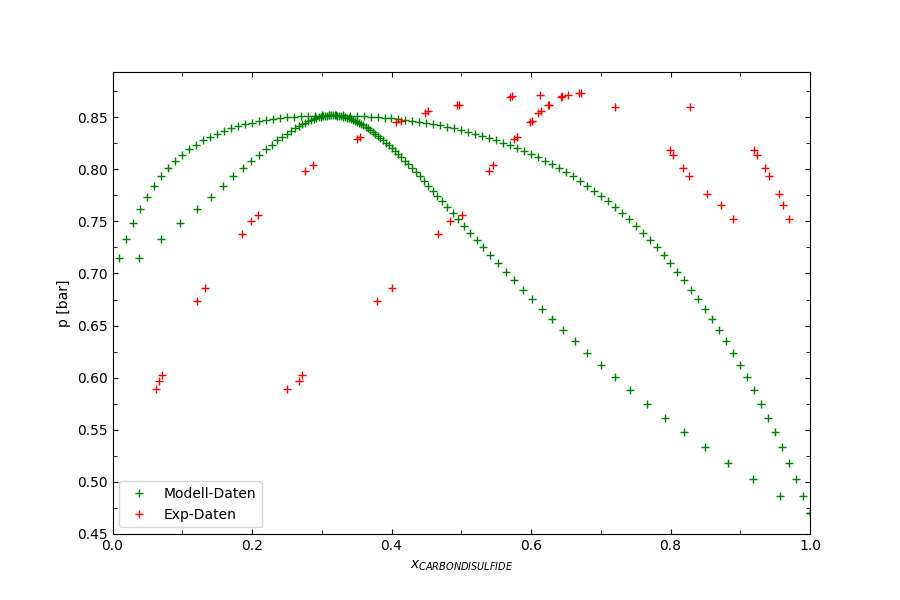
\includegraphics[scale=0.6]{CARBON DISULFIDE_ACETONE_isotherm_308.32_}
	\caption{Isothermes Phasengleichgewicht bei $ 308$.$32$ K für das Stoffgemisch Kohlenstoffdisulfid|Aceton}
	\label{fig: phase_eq_fehler}
\end{figure}

Die Daten des Experiments und die des Modells sind für unterschiedliche Komponenten dargestellt. Dies macht deutlich, dass eine Lagebestimmung sowohl der experimentellen als auch der Modelldaten notwendig ist, um eine korrekte Orientierung im Diagramm zu gewährleisten. Mit Lagebestimmung ist hier die Bestimmung der Komponente der x-Achse gemeint. Nur wenn diese für Experiment und Modell übereinstimmt können korrekte Abweichungen ermittelt werden. Das Vorgehen zur Bestimmung der x-Achsen Komponente ist in \autoref{fig: phasediagrammlage} dargestellt.

\begin{figure}[htb]
	\centering
	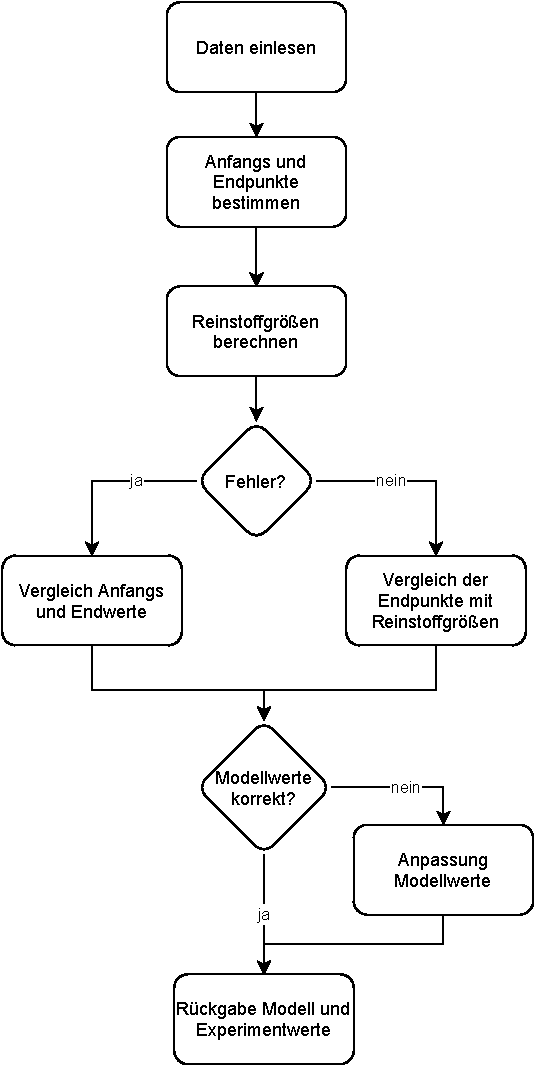
\includegraphics[scale=0.85]{phasendiagrammlage}
	\caption{Vorgehen bei der Lagebestimmung der Modelldaten im Phasendiagramm}
	\label{fig: phasediagrammlage}
\end{figure}

Als erstes werden die experimentellen und vom Modell berechneten Daten an die Methode übergeben und von dieser eingelesen. Als nächstes werden die Endpunkte bestimmt. Als Endpunkte werden hier die Punkte mit dem größten und kleinsten Molenbruch definiert. Im Idealfall liegen in den experimentellen Daten Datenpunkte bei $x = 0$ und $ x = 1$ vor oder es gibt Punkte, welche nicht weit von diesen Punkten entfernt liegen. Diese Punkte können mit den Reinstoffgrößen der beteiligten Komponenten verglichen werden, um die Lage im Diagramm eindeutig zu definieren. Die Reinstoffwerte werden ebenfalls mit der \texttt{TREND} Routine \texttt{TREND\_EOS\_FIT} berechnet. Sofern die Berechnung erfolgreich verläuft, wird der Abstand der Endpunkte von den berechneten Reinstoffwerten ermittelt und basierend darauf entschieden, ob die Lage der  Modelldaten zu den experimentellen Daten passt oder nicht. Nach diesem Schritt ist klar für welche Komponente die experimentellen Daten und für welche Komponente die Modelldaten vorliegen. 

Wenn die Berechnung einen Fehler erzeugt, werden anstatt der Reinstoffwerte die Endpunkte des Modells im Vergleich verwendet. In diesem Fall kann nur über die Lage des Experiments im Vergleich zu der des Modells entschieden werden. Hier kann es zu Fehlern kommen, wenn nur wenige experimentelle Datenpunkte zur Verfügung stehen oder diese Punkte nur über einen kleinen Bereich verteilt sind. Eine ausführlichere Fehlerbeschreibung und eventuelle Verbesserungsmöglichkeiten werden in \autoref{chap: fehler} beschrieben. 

Wenn die Lage der Modelldaten zu der Lage der experimentellen Daten passt, werden diese, so wie sie der Methode übergeben worden sind, wieder zurückgegeben. Die Entscheidung ob die Lagen übereinstimmen wird anhand der Komponente der x-Achse getroffen. Sind Modell und Experiment dahingehend identisch stimmen die Lagen überein. Sollten die Lagen nicht zueinander passen, werden die Molenbrüche der Modelldaten invertiert und die neuen Modelldaten mit den experimentellen Daten zurückgegeben. Die Methode, welche für die Lageerkennung zuständig ist befindet sich in der Datei \texttt{check\_phase\_eq\_direction.py}, da diese sowohl in der Klasse \texttt{model} als auch in der Klasse \texttt{compare} benötigt wird.

In den nun korrekt orientierten Datensätzen des Modells und Experiments wird der zu einem experimentellen Datenpunkt gehörende Punkt des Modells gesucht. Für diesen Punkt gilt, dass für diesen der variable Parameter, welcher auf der y-Achse des Phasengleichgewichtsdiagramms dargestellt ist, der Wert des Modells und des Experiments möglichst gleich sein soll. Im Falle eines isothermen Phasengleichgewichts wie in \autoref{fig: phasediagrammlage} zu sehen, ist dieser variable Parameter der Druck $ p $ in bar. Analog wird im Falle eines isobaren Phasengleichgewichts nach der gleichen Temperatur $ T $ in K gesucht. Da die Werte des Modells und die des Experiments nicht genau übereinstimmen, wird hier der Einfachheit halber der Punkt des Modells mit dem geringsten Abstand zum Punkt des Experiments verwendet. Eine schematische Darstellung des Verfahrens ist in \autoref{fig: phasendiagrammsuche} dargestellt. 

\begin{figure}[htb]
	\centering
	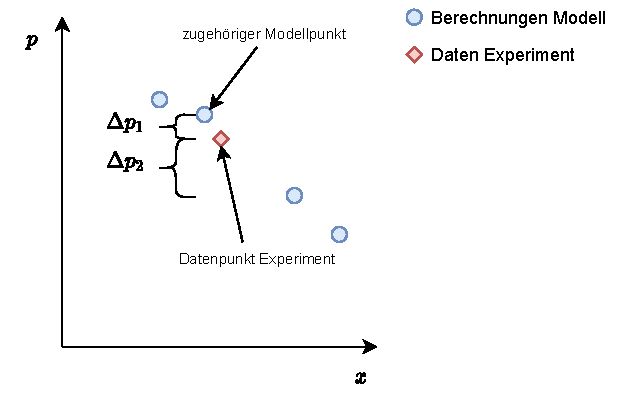
\includegraphics[scale=1.1]{phasendiagrammsuche}
	\caption{Schematische Darstellung der Zuordnung von Modelldatenpunkten zu experimentellen Datenpunkten für ein Phasendiagramm}
	\label{fig: phasendiagrammsuche}
\end{figure}

Da die Druckdifferenz $\Delta p_1$ kleiner $ \Delta p_2$ ist, wird der gekennzeichnete Modellpunkt dem experimentellen Datenpunkt zugeordnet. Da die Daten des Modells und die des Experiments meistens sehr eng beieinander liegen, wurde bisher auf eine Interpolation verzichtet. Liegen Punkte des Experiments oberhalb oder unterhalb der Modelldaten, wie beispielsweise in \autoref{fig: phase_eq_datenausschluss} zu sehen, werden diese aus der Bewertung ausgeschlossen. 

\begin{figure}[htb]
	\centering
	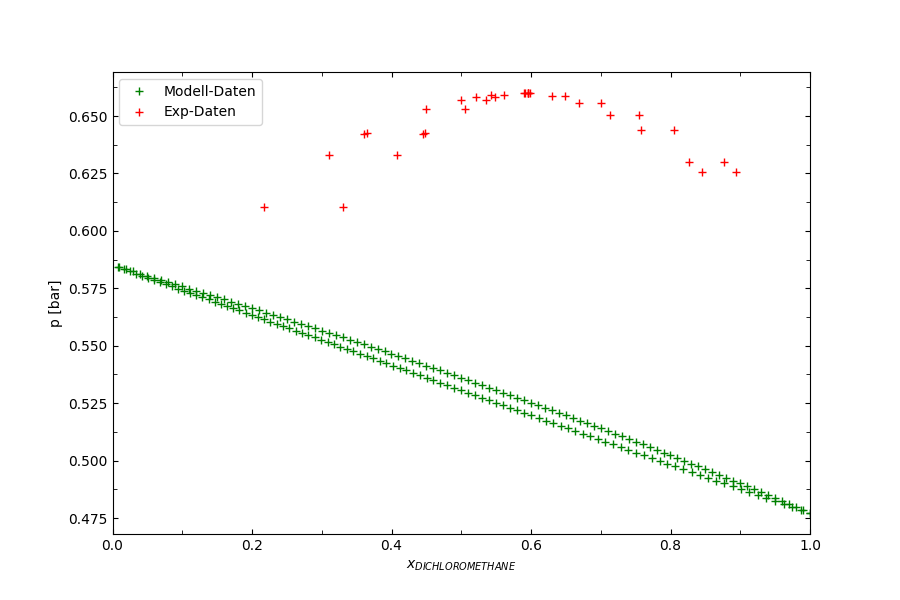
\includegraphics[scale=0.48]{DICHLOROMETHANE_CARBON DISULFIDE_isotherm_298.15_}
	\caption{Isothermes Phasengleichgewicht bei $ 298$.$15$ K für das Stoffgemisch Dichlormethan|Kohlenstoffdisulfid}
	\label{fig: phase_eq_datenausschluss}
\end{figure}

Anschließend werden die entsprechenden Molenbrüche der Flüssigkeit $x$ und der Gasphase $y$ für den Punkt des Experiments und den gefunden Punkt des Modells zwischengespeichert. Sind alle Messreihen durchsucht worden, werden die zwischengespeicherten Molenbrüche miteinander verglichen und bewertet.

\subsection{Bewertung azeotroper Punkt}

Für die Bewertung des azeotropen Punkts werden die Modelldaten dieses Punktes benötigt. Da es keine direkte Berechnungsmethode in \texttt{TREND} für diese Größe gibt, wird dieser aus den berechneten Phasengleichgewichtsdaten extrahiert. Die Methode durchsucht nur diejenigen Stoffgemische, bei denen in den experimentellen Phasengleichgewichten azeotrope Punkte vermerkt wurden. Da der azeotrope Druck als Bewertungsgröße definiert ist, werden nur isotherme Phasengleichgewichte betrachtet, da nur hier der Druck berechnet und verändert wird. Um den azeotropen Punkt zu finden, wird nach dem Maximum bzw. Minimum des Drucks in den Daten gesucht und die zugehörigen Molenbrüche gespeichert. Azeotrope Gemische können als Druckmaximumazeotrope wie in \autoref{fig: durckmaximumazeotrop} dargestellt oder als Druckminimumazeotrope wie in \autoref{fig: druckminimumazeotrop} zu sehen auftreten. In beiden Fällen wird die Abweichung des vom Modell berechneten Drucks und die Abweichung der vom Modell berechneten Zusammensetzung $x$ von den experimentellen Werten bewertet. Eine separate Bewertung der Zusammensetzung der Dampfphase $y$ ist nicht notwendig, da diese am azeotropen Punkt gleich der der Flüssigphase ist. 

\begin{figure}[htb]
	\centering
	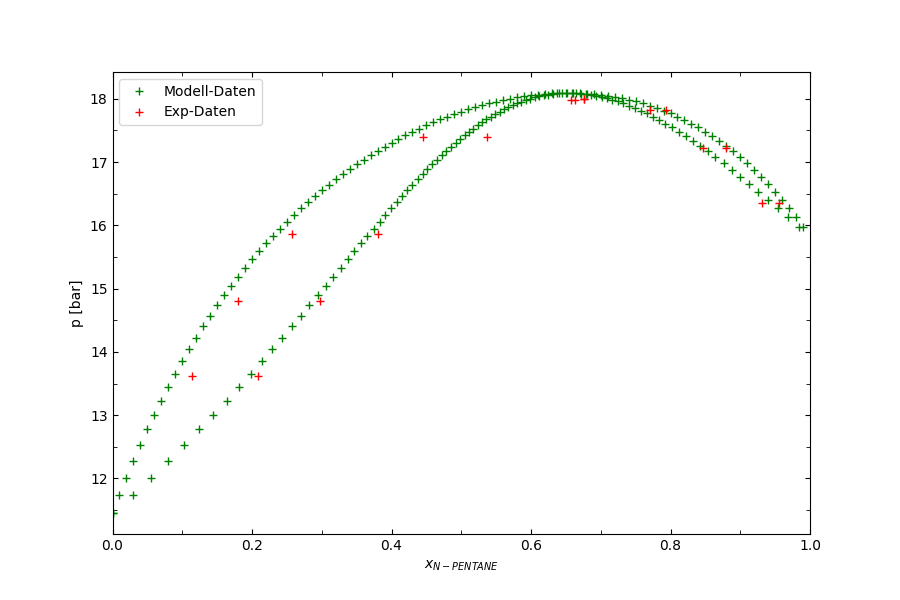
\includegraphics[scale=0.55]{ACETONE_N-PENTANE_isotherm_422.6_}
	\caption{Isothermes Phasengleichgewicht bei $ 422$.$6$ K für das Stoffgemisch Azeton|n-Pentan}
	\label{fig: durckmaximumazeotrop}
\end{figure}

\begin{figure}[hbt]
	\centering
	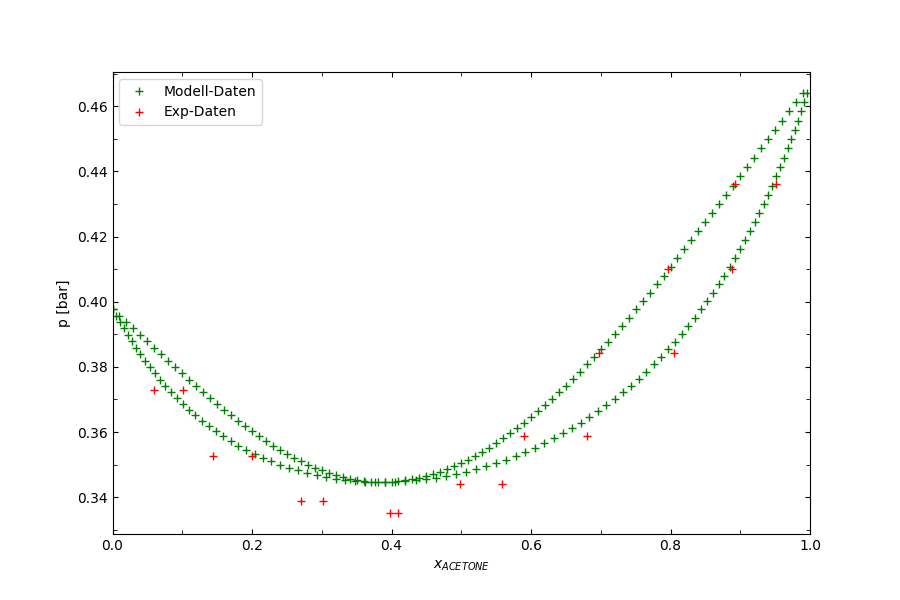
\includegraphics[scale=0.55]{CHLOROFORM_ACETONE_isotherm_308.15_}
	\caption{Isothermes Phasengleichgewicht bei $ 308$.$15$ K für das Stoffgemisch Chloroform|Azeton}
	\label{fig: druckminimumazeotrop}
\end{figure}

\subsection{Bewertung weiterer Zustandsgrößen}

Die weiteren Zustandsgrößen des Gemisches wie die des kritischen Punkts $ p_{\mathrm{c}}$ und $ x_{\mathrm{c}}$, sowie die 3-Phasen Zustandsgrößen $p_{\mathrm{LLV}}$ und $z_{\mathrm{LLV}}$ können vom Modell bisher nicht direkt berechnet werden.

Aufgrund der fehlenden Daten des Modells können für diese Größen bisher keine Noten berechnet werden, sodass diese in der Bewertung des thermodynamischen Modells bisher nicht berücksichtigt werden.

\end{document}
